\documentclass{beamer}
\usetheme{Warsaw}

\fontfamily{pag}
\usepackage{libertine}
\renewcommand*\familydefault{\sfdefault}

\setlength{\parskip}{1em}

\setbeamercolor{normal text}{fg=white,bg=black!90}
\setbeamercolor{structure}{fg=white}

\setbeamercolor{alerted text}{fg=red!85!black}

\setbeamercolor{item projected}{use=item,fg=black,bg=item.fg!35}

\setbeamercolor*{palette primary}{use=structure,fg=structure.fg}
\setbeamercolor*{palette secondary}{use=structure,fg=structure.fg!95!black}
\setbeamercolor*{palette tertiary}{use=structure,fg=structure.fg!90!black}
\setbeamercolor*{palette quaternary}{use=structure,fg=structure.fg!95!black,bg=black!80}

\setbeamercolor*{framesubtitle}{fg=white}

\setbeamercolor*{block title}{parent=structure,bg=black!60}
\setbeamercolor*{block body}{fg=black,bg=black!10}
\setbeamercolor*{block title alerted}{parent=alerted text,bg=black!15}
\setbeamercolor*{block title example}{parent=example text,bg=black!15}

\usepackage{grffile} %for underscores in file names
\usepackage{gensymb} % degree
\title{The Science of Brewing:}
\subtitle{How 4 simple ingredients become the best beverage in the world \newline \newline Part 1: Barley}
\date{\footnotesize{\today}}
\author{Nick Waters}
\institute{Department of Microbiology\\
School of Natural Sciences\\
National University of Ireland, Galway}

\begin{document}
\maketitle
\begin{frame}
\frametitle{Ingredients}
\begin{enumerate}
\item Barley
\item Hops
\item Water
\item Yeast
\end{enumerate}
\end{frame}

% barley
\begin{frame}
\frametitle{Barley}
% \framesubtitle{Test Frame}
\begin{itemize}
\item \textit{Hordeum vulgare}
\item 4th Most Produced Grain
\end{itemize}
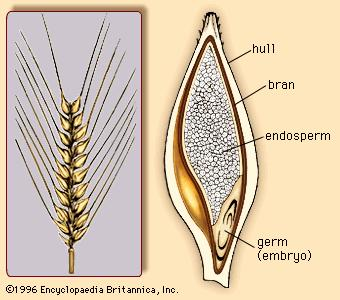
\includegraphics[width=.4\linewidth]{./brewing/619-004-B70AF7D8.jpg}
\hspace{5mm}
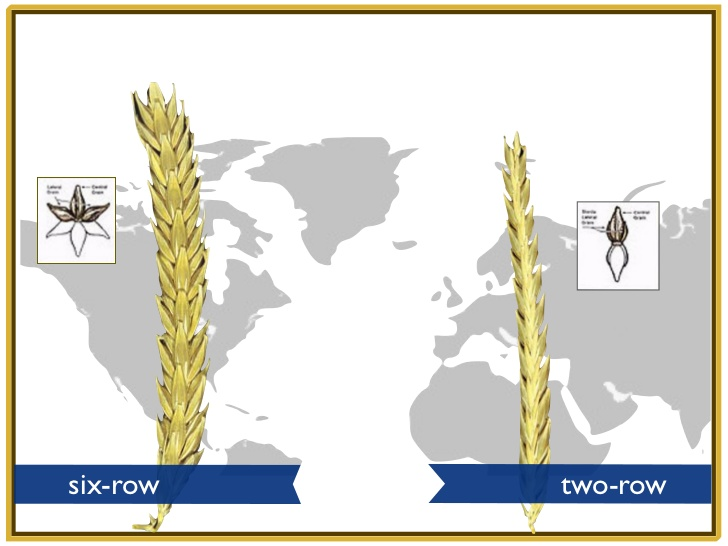
\includegraphics[width=.47\linewidth]{./brewing/barleyrow.jpg}
\end{frame}

% two vs 6
\begin{frame}
\frametitle{2-row vs 6-row }
% \framesubtitle{Test Frame}
\begin{table}[]
\centering
\label{tworow}
\resizebox{\textwidth}{!}{
  \begin{tabular}{lcc}
                  & Two Row    & Six Row                \\
    \hline
    Lineage           & ancestral  & derived                \\
    vrs1 locus        & WT         & mutant                 \\
    Where             & old world  & new world              \\
    Protein vs Carbs  & more sugar & more protein/enzymes   \\
    Starch Conversion & less yield per head & 2-4\% lower extraction \\
    Germination Time & 2 days     & 4 days                 \\
    Diastic Power     & ++         & +++
\end{tabular}}
\end{table}
\end{frame}

%malting
\begin{frame}
\frametitle{Malting}
\begin{itemize}
  \item Dry: Grains are dried to encourage natural dormancy
\item Steep:  Hot water is added to grains to rehydrate the kernals for 2-3 days, encourage sprouting
\item Germinate: Embryo starts making enzymes and converting start reserves
\item Kiln: Germination is halted to preserve optimal sugar and enzume content
\end{itemize}
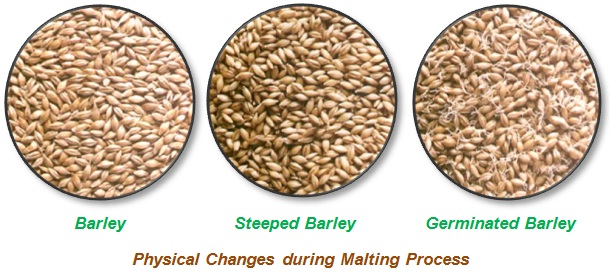
\includegraphics[width=.7\linewidth]{./brewing/malting.jpg}
\end{frame}




% types of malt
\begin{frame}
  \frametitle{Malt Types}
  \vspace*{-5mm}
\begin{table}[]
\centering
\label{malts}
\resizebox{\textwidth}{!}{
  \begin{tabular}{llll}
  Malt Type     & Lovibond & Modification & Charactaristics                      \\
  \hline
  Lager         & 2        & ++   & neutral                     \\
  Pale Ale      & 3        & ++   & general purpose                       \\
  Wheat         & 3        & ++   & wheaty                      \\
  Rye           & 3        & ++   & flavorful, spicy            \\
  Biscuit       & 25       & ++   & bready                      \\
  Victory       & 25       & ++   & bready/nutty                \\
  Munich        & 10       & ++   & oktoberfest                 \\
  Vienna        & 4        & ++   & bocks                       \\
  Carapils      & 3        & ++   & texture                     \\
  Caramel 10    & 10       & +    & honey                       \\
  Caramel 40    & 40       & +    & light caramel               \\
  Caramel 60    & 60       & +    & full caramel                 \\
  Caramel 120   & 120      & +    & bittersweet caramel         \\
  Special B 220 & 220      &      & plums, nutty bitter caramel \\
  Chocolate     & 400      &      & bittersweet chocolate       \\
  Black Patent  & 580      &      & charcoal                    \\
  Roast Barley  & 550      &      & coffee, Guinness
\end{tabular}}
\end{table}
\end{frame}



%%%% MAsh
\begin{frame}
\frametitle{Mash}
% \framesubtitle{Test Frame}
\begin{enumerate}
\item Protein Rest 30-40\degree: Encourages proteases
\item Mashing 60-70\degree: Encourage $\alpha$ and $\beta$ amylases
\item Hot Crash 75\degree: Denaturation of Enzymes
\end{enumerate}
\end{frame}


\begin{frame}
\frametitle{Enzymes}

  \begin{table}[]

\centering
\caption{Mash Enzymes and Their Optimal Temperatures}
\label{enz}
\resizebox{\textwidth}{!}{
  \begin{tabular}{llll}
    Enzyme & Temp (\degree C)&  pH Range & Function \\
    \hline
    Debranching (var.) & 35-45\degree & 5.0-5.8 & Solubilization of starches. \\
    $\beta$ Glucanase & 35-45\degree & 4.5-5.5 & Best gum breaking rest. \\
    Peptidase & 45-55\degree & 4.6-5.3 & Produces Free Amino Nitrogen (FAN). \\
    Protease & 45-55\degree & 4.6-5.3 & Breaks up large proteins that form haze. \\
    $\beta$ Amylase & 55-66\degree & 5.0-5.5 & Produces maltose. \\
    $\alpha$ Amylase & 67-72\degree & 5.3-5.7 & Produces a variety of sugars, including maltose.
\end{tabular}}
\end{table}
\end{frame}



\begin{frame}
\frametitle{After the Mash: Lautering}
\begin{itemize}
\item Goal is to achieve maximum extraction of sugars
\item Temp $>$ 77\degree  leads to tannin extraction from hulls
  \item Sparging is the addition of more water to rinse grains
\item Aim for volume about 1.4x desired final volume
\item Grain husks help filter
\end{itemize}
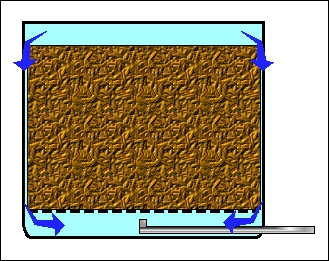
\includegraphics[width=.41\textwidth]{./brewing/lauter1.jpg}
\hspace*{3mm}
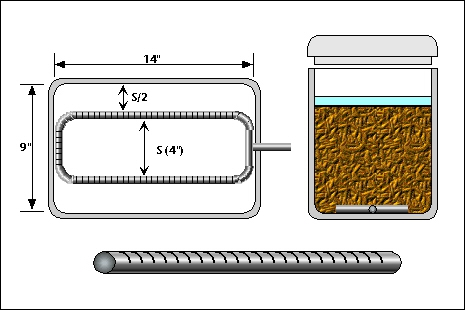
\includegraphics[width=.488\textwidth]{./brewing/lauter2.jpg}
\end{frame}

\section{Our Brew}
\begin{frame}
  \frametitle{BGCP Guidelines: 9E. Strong Scotch Ale}
  {\footnotesize

\textbf{Aroma:} Deeply malty, with caramel often apparent. Peaty, earthy and/or smoky secondary aromas may also be present, adding complexity. Caramelization. Hops very low to none.

\textbf{Appearance:} Light copper to dark brown color, often with deep ruby highlights. Clear. Usually has a large tan head, which may not persist in stronger versions.

\textbf{Flavor:} Richly malty with kettle caramelization often apparent. Hints of roasted malt or smoky flavor may be present, as may some nutty character, all of which may last into the finish. Hop flavors and bitterness are low to medium-low, so malt impression should dominate.  Esters may suggest plums, raisins or dried fruit. The palate is usually full and sweet, but the finish may be sweet to medium-dry (from light use of roasted barley).

}
\end{frame}
\begin{frame}
  \frametitle{BGCP Guidelines: 9E. Strong Scotch Ale, cont.1}
  {\footnotesize

\textbf{Mouthfeel:} Medium-full to full-bodied, with some versions (but not all) having a thick, chewy viscosity. A smooth, alcoholic warmth is usually present and is quite welcome since it balances the malty sweetness. Moderate carbonation.

\textbf{Overall Impression:} Rich, malty and usually sweet, which can be suggestive of a dessert. Complex secondary malt flavors prevent a one-dimensional impression. Strength and maltiness can vary.

\textbf{Comments:} Also known as a “wee heavy.” Fermented at cooler temperatures than most ales, and with lower hopping rates, resulting in clean, intense malt flavors. Well suited to the region of origin, with abundant malt and cool fermentation and aging temperature. Hops, which are not native to Scotland and formerly expensive to import, were kept to a minimum.
}
\end{frame}
\begin{frame}
  \frametitle{BGCP Guidelines: 9E. Strong Scotch Ale, cont. 2}
  {\footnotesize

\textbf{Ingredients:} Well-modified pale malt, with up to 3\% roasted barley. May use some crystal malt for color adjustment; sweetness usually comes not from crystal malts rather from low hopping, high mash temperatures, and kettle caramelization. A small proportion of smoked malt may add depth, though a peaty character (sometimes perceived as earthy or smoky) may also originate from the yeast and native water. Hop presence is minimal, although English varieties are most authentic. Fairly soft water is typical.

\textbf{Commercial Examples:} Traquair House Ale, Belhaven Wee Heavy, McEwan's Scotch Ale, Founders Dirty Bastard, MacAndrew's Scotch Ale, AleSmith Wee Heavy, Orkney Skull Splitter, Inveralmond Black Friar, Broughton Old Jock, Gordon Highland Scotch Ale, Dragonmead Under the Kilt}
\end{frame}

\begin{frame}
\frametitle{Microsoc Brew \#2: Scotch Wee Heavy}
The Grains:
\begin{itemize}
\item 7kg Marris Otter (2row)
\item 250g Roasted Barley
\end{itemize}
The Mash:
\begin{itemize}
\item 30min @ 40\degree
\item 40min @ 60\degree
\item 20min @ 70\degree
\end{itemize}
\end{frame}

\begin{frame}
\frametitle{Microsoc Brew \#2: Scotch Wee Heavy}

The Boil:
\begin{itemize}
\item 3/4 Volume for 60mins
\item 1/4 Volume for 30mins (kettle carmelization)
\item 75g Fuggle hops @ 60mins
\item 25g Fuggle hops @ flameout
\end{itemize}
The Fermentation:
\begin{itemize}
\item Starter from 3/4 yeast (safbrew T-58)
\item Starter from 1/4 yeast (safbrew T-58) after 2 weeks
\end{itemize}

Estimated Final ABV: 9.0\%

\end{frame}



\begin{frame}
  \frametitle{source}
  \begin{enumerate}
  \item http://howtobrew.com/book/section-3/how-the-mash-works/mashing-defined
  \item https://www.britannica.com/plant/barley-cereal
  \item https://www.slideshare.net/kourtney-kathryn/advanced-foods-presentation-beer
  \item https://www.integrowmalt.com/about-integrow/malting-barley-storage.html
  \item http://www.morebeer.com/brewingtechniques/bmg/schwarz.html

  \end{enumerate}
  \end{frame}

\end{document}